\documentclass{kththesis}

% remove this if you are using XeLaTeX or LuaLaTeX
\usepackage[utf8]{inputenc}

% Use natbib abbreviated bibliography style
\usepackage[square,numbers]{natbib}

\usepackage{amsmath,amsthm,amssymb}
\usepackage{graphicx}
\usepackage{multicol}

\usepackage{subcaption}
\usepackage[section]{placeins}

\usepackage{tikz}

\bibliographystyle{unsrtnat}

%\usepackage{natbib}
%\bibliographystyle{agsm}

\usepackage{lipsum} % This is just to get some nonsense text in this template, can be safely removed

\title{Predicting Game Level Difficulty Using Deep Neural Networks}
\alttitle{Uppskattning av spelbanors svårighetsgrad med djupa neurala nätverk}
\author{Sami Purmonen}
\email{purmonen@kth.se}
\supervisor{Karl Meinke}
\examiner{Olov Engwall}
\programme{Master in Computer Science}
\school{School of Computer Science and Communication}
\date{\today}


\begin{document}

% Title page
\flyleaf

\begin{abstract}
We explored the usage of Monte Carlo tree search (MCTS) and deep learning in order to predict game level difficulty in Candy Crush Saga (Candy) measured as number of attempts per success. A deep neural network (DNN) was trained to predict moves from game states from large amounts of game play data. The DNN played a diverse set of levels in Candy and fitted a model to predict human difficulty from bot difficulty. We compared our results to an MCTS bot. Our results indicate that the DNN can make estimations of game level difficulty comparable to MCTS in shorter time.
\end{abstract}

\clearpage

\begin{otherlanguage}{swedish}
  \begin{abstract}
  Vi utforskade användning av Monte Carlo tree search (MCTS) och deep learning för att uppskatta banors svårighetsgrad i Candy Crush Saga (Candy). Ett deep neural network (DNN) tränades för att förutse speldrag från spelbanor från stora mängder speldata. DNN:en spelade en varierad mängd banor i Candy och en modell byggdes för att förutse mänsklig svårighetsgrad från DNN:ens svårighetsgrad. Resultatet jämfördes med MCTS. Våra resultat indikerar att DNN:ens kan göra uppskattningar jämförbara med MCTS men på substantiellt kortare tid.
  \end{abstract}
\end{otherlanguage}

\cleardoublepage

\tableofcontents


% This is where the actual contents of the thesis starts
\mainmatter

\chapter{Introduction}
Playing games can be fun, but only if the game levels are not too hard nor too easy. Predicting how difficult a game level is before releasing it to players however is difficult. A common method is to let level designers or explicit play testers play a level many times and make a guess. This approach is slow and unreliable.

It is useful for game companies and level designers to have fast and accurate tools for predicting game level difficulty automatically. It is especially important for games that continuously release new levels such as King's Candy Crush Saga (Candy). It would allow level designers to tweak a level many times before release to ensure that it has an appropriate difficulty. 

\section{Bot}
One automated way of predicting game level difficulty is to create a program, a bot, that plays the game according to some strategy. The bot can play a level many times and estimate how difficult it is for the bot according to a difficulty measurement such as the numbers of attempts per success. If we let the bot play many levels and estimate the bot difficulty for each of those we can compare that to how difficult those levels were for humans and try to relate the bot difficulty with human difficulty.  If it is the case that when a level is comparably hard for a human, it is also comparably hard for the bot, and when it is comparably easy for a human it is comparably easy for the bot, then we might be able to create a useful regression model to predict human difficulty from bot difficulty. The difficulty of new levels can then be predicted by playing it many times with the bot to measure the bot difficulty and then predicting human difficulty from bot difficulty using the prediction model. There are many methods to create a strategy.

\subsection{Handmade Heuristic}
One strategy the bot can use is a handmade heuristic that ranks the available moves and then select the best one. The heuristic can look at the current game state to judge how desirable each available move is. The drawback of this approach is that it is not general or maintainable. When the game changes, for example a new game element is introduced, the heuristic need to be updated. A new heuristic must be created for each game.

\subsection{Monte Carlo tree search}
A much more general approach is the Monte Carlo tree search (MCTS). Instead of creating a large set of rules determining how desirable a move is, MCTS uses simulations. MCTS will perform each move many times and play to the end and estimate how often it leads to success. This requires zero knowledge of the game and can automatically handle when the game changes or be used on a completely new game. The drawback of MCTS is that it is slow since it needs to simulate the game play many times.

\subsection{Deep Neural Network}
Machine learning could be used to rank moves from game states as well, essentially learning a heuristic from data. If a large dataset containing game states and moves is available it can be used in supervised learning to train a classifier that predicts which move to select from any given game state. Deep neural networks (DNNs) is one machine learning algorithm that can be used for classification and has made major breakthroughs in image recognition, machine translation and games. Using a DNN to predict moves from game states would be much faster than MCTS because it does not need to make simulations and it is also general since only a new dataset is needed to learn a new game. The question remains whether it also is accurate. That is what will be explored in this thesis. Table \ref{fig:bot_properties} shows how the methods hypothetically compare to each other.

\begin{table}
\caption{Bot properties, the properties of the DNN are hypothetical}
\centering
\begin{tabular}{l{c}rr}
\hline
Bot type&Speed&Accurate&General\\
\hline
MCTS&&\checkmark&\checkmark\\
Handmade heuristic&\checkmark&\checkmark&\\
DNN&\checkmark&\checkmark&\checkmark\\
\hline
\end{tabular}
\label{fig:bot_properties}
\end{table}

\section{Problem}
In this thesis we explore the problem of predicting game level difficulty in the context of Candy Crush Saga with a DNN trying to discover an approach that is fast, accurate and general. We want to know if predictions of game level difficulty can be improved using a bot based on a neural network instead of Monte Carlo tree search, which is what King already has available.

\section{Delimitation}
We restrict ourselves to one of King's games, Candy Crush Saga, and using training data generated by an MCTS bot.

\chapter{Relevant Theory}
In this chapter we provide the  theoretical foundation that our work is based on. We take a deeper look into how neural networks work and how they are trained since it is the most important part of this thesis and where a large part of the work has been invested.

\section{Related Work}
The primary source of inspiration comes from  Google Deepminds AlphaGo paper and Erik Poromaas master thesis. Other sources of inspiration comes from image recognition since the problem of predicting moves from game states can be seen as an image recognition problem. Broader sources of inspiration is anything related to machine learning or AI in games.\\

In "Mastering the game of Go with deep neural networks and tree search" a computer Go program using a combination of supervised learning, reinforcement learning and MCTS is invented. It is the first computer Go program that could beat professional Go players on a full-sized board \cite{alphaGo2016}. Our work is heavily inspired by the supervised learning part from AlphaGo but we use it to predict game difficulty instead of creating the strongest possible bot. \\

In "Crushing Candy Crush" Erik Poromaa predicts game level difficulty in Candy Crush using MCTS. He finds that this method outperforms previous state-of-the-art methods of manual testing \cite{poromaa2016}. We compare our results with the MCTS bot he created. \\

In "ImageNet Classification with Deep Convolutional Neural Networks" a large deep convolutional neural network is trained on millions of high-resolution images substantially improving previous state-of-the-art in the ImageNet LSVRC-2010 contest \cite{krizhevsky2012imagenet}. Even though the aim here is to decide what kind of object is visible in an image it is similar to our problem since the game board can be seen as an image with many more channels than 3 as for RGB and the object we are trying to identify is one of the possible 144 moves, therefore a convolutional neural network is suitable for our problem as well. \\

In "Move Evaluation in Go Using Deep Convolutional Neural Networks" a 12-layer deep convolutional neural network  is trained on a dataset of human professional Go players  to predict moves. It predicts professional moves with 55\% accuracy  and could beat traditional search programs without any search \cite{goMoveEvaluation2014}. This paper inspired AlphaGo and is very similar to what we have done in that they create a DNN bot for Go based on only supervised learning, however we take one step further and use the bot the predict game level difficulty.\\

In "Predicting moves in chess using convolutional neural networks" a deep convolutional neural network is trained to predict moves from game states in chess. The problem with chess is that a move is defined by the position a piece is moved from and the position it is moved so there are 64*64 or 4096 different moves that a classifier needs to distinguish between. In order to reduce the number of moves they used a novel approach of creating two separate networks, one which predicts which piece to move and one which predicts where to move it thus reducing the class space to 64 for each network. They managed to predict which piece to move with 38.3\% accuracy \cite{oshripredicting}. Their aim to predict moves is the same as ours except we did not need to be creative in order to reduce the class space as the number of moves in our problem is 144 which is tractable, in Go there are 361 moves. \\

In "Playing Atari with Deep Reinforcement Learning" a  model based on convolutional neural networks and reinforcement learning was created to play seven Atari 2600 games. It outperformed all previous approaches on six of the games  and  performs better than a human expert on three of them \cite{mnih2013playing}. A similar reinforcement method would be interesting to apply on our problem but we decided to go for supervised learning instead because we think the best way to predict game level difficulty would be to create a bot that mimics human players. We could not do that since we did not have human play data at the time this thesis was written but could do that in the future. \\

\section{Monte Carlo Tree Search}
It is common to use different game tree search algorithms when creating agents playing games. The Minimax algorithm is a tree search algorithm that has reached state-of-the-art performance in games such as Chess, Checkers and Othello where good heuristics for evaluating game states are available \cite{alphaGo2016}. In games such as Go where it is hard to come up with heuristics, MCTS has instead been the most successful game search algorithm until AlphaGo \cite{goMoveEvaluation2014}.

\begin{figure}
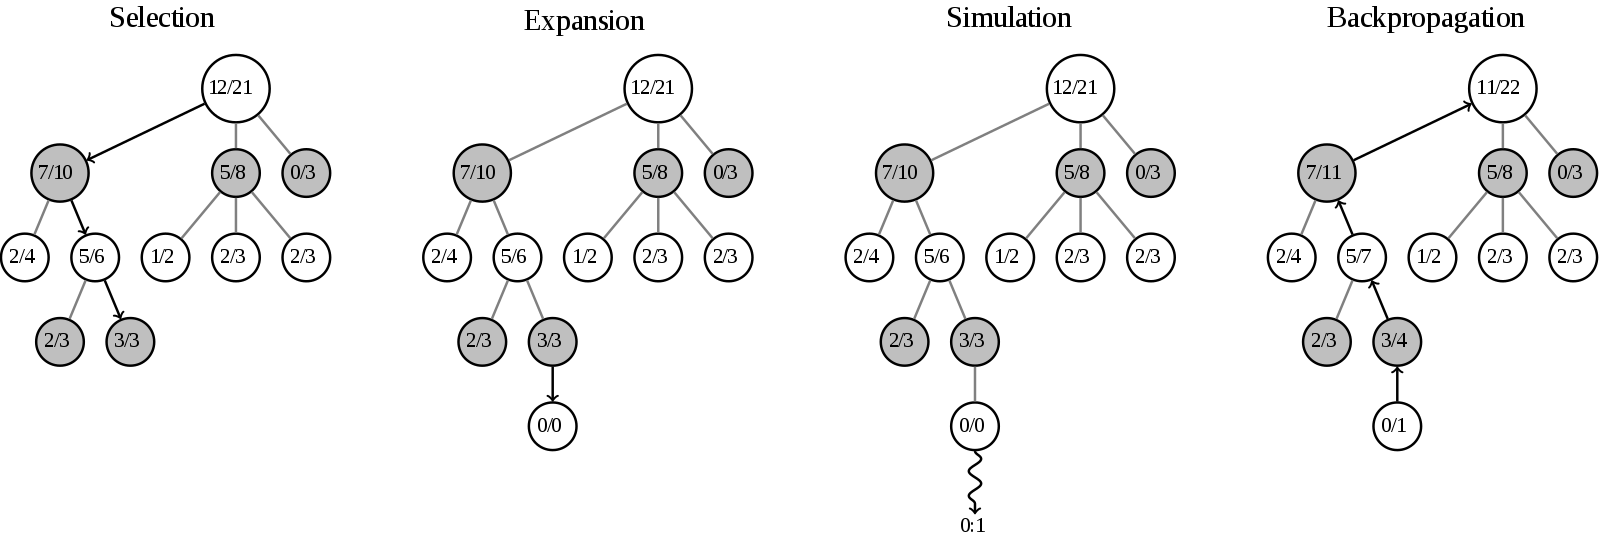
\includegraphics[width=\textwidth]{images/mcst.png}
\caption{The steps in MCTS}
\label{fig:mcts-steps}
\end{figure}

MCTS determines the best possible action from a state by expanding a search tree using random sampling. It can be applied to any game with finite length and finite number of moves. Each action is a node in the search tree and records the number of wins and visits which is used to guide the search tree towards better moves. It consists of four steps performed iteratively: selection, expansion, simulation and backpropagation as Fig \ref{fig:mcts-steps}. Doing this many times converges to optimal play \cite{kocsis2006bandit}.

\subsubsection{Selection}
The selection starts at current state which is the root of the search tree then it selects child nodes until it reaches a leaf node. The selection of child nodes is done in a way that will expand the tree towards the most promising move using the number of wins and visits but also allows exploration.

\subsubsection{Expansion}
When a leaf node is reached, the search tree is expanded with a new child node unless the game has reached the end.

\subsubsection{Simulation}
The game is simulated to the end by randomly selecting actions.

\subsubsection{Backpropagation}
The result of the playout is backpropagated through all visited nodes back to the root updating the number of wins and visits.


\section{Machine Learning}
Machine learning  encompasses algorithms that learn from experience. Supervised learning is the most common form of machine learning. A supervised learning algorithm learn a function $F: \mathbb{R}^{N} \rightarrow \mathbb{R}^{M}$ from a training set of examples of such mappings and then its predictions on unseen data becomes better, meaning that it is generalizing. 

\subsection{Classification}
Classification means to assign a class $c \in C$ from a finite set  of classes to an input of features. For example, we could have a classifier that takes as input  the height and weight of a person and outputs $c \in \{Male, Female\}$. Given a dataset of persons weight and height  labeled with female or male  a  learning algorithm could generate a classifier that predicts the gender of persons.  The purpose of the classifier is to use it on unseen data so the goal during training is to train a classifier that generalizes to unseen data.

\newcommand{\argmax}[1]{\underset{#1}{\operatorname{arg}\,\operatorname{max}}\;}
\subsubsection{Data representation}
\label{sec:machine_learning:data_representation}
The input to a classifier is a vector $X \in \mathbb{R}^{n}$ where $n$ is the  number of features.
The output of the classifier is a vector $Y \in \mathbb{R}^{c}$ where $c$ is the number of classes and $Y_{i}$ is the score of class $i$. The predicted class is $\argmax{i}Y_{i}$. $Y$ can be normalized so that $\sum_{i}Y_{i}=1$ making it a conditional probability distribution over the given classes $P(i|X)=Y_i$ using the softmax function as shown in equation \ref{eq:softmax}. 

\begin{equation}
\label{eq:softmax}
Y_i=\frac{e^{Y_i}}{\sum_j{e^{Y_j}}}
\end{equation}

This is the way we will think of classification in this thesis. It is a way to generate a probability distribution over all possible classes from an input vector.

\subsection{Artificial Neural Network}
\begin{figure}
\centering
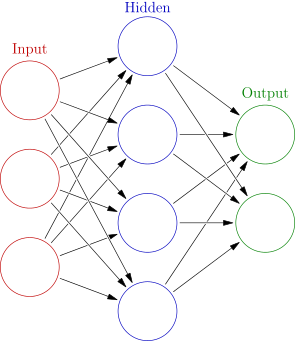
\includegraphics[width=0.5\textwidth]{images/ann.png}
\caption{Fully-connected artificial neural network with one hidden layer}
\label{fig:ann}
\end{figure}

A neural network is a supervised learning algorithm. We will discuss how it is used for the task of classification. A neural network consists of layers  of neurons connected to each other with weights. We will discuss feed-forward neural networks where neurons at layer $i+1$ are only connected to neurons at layer $i$, as shown in Fig \ref{fig:ann}. Neural networks where neurons have backward connections are called recurrent neural networks and are useful in speech recognition where time is important.  Artificial neurons are loosely modeled after biological  neurons inside the brain. However, we will  think of them as mathematical units since the connection to biology does not ease the understanding of  how they work unless one has a background in biology.

\subsubsection{From Input to Output}
A neural network used for classification takes an input vector $X \in \mathbb{R}^{n}$ and outputs a vector $Y \in \mathbb{R}^{c}$ representing a probability distribution over the possible classes, as described in Section \ref{sec:machine_learning:data_representation}. What is different between a neural network and other classifiers is how it does it. That is what we will discuss next. 

\subsubsection{Work of the Neuron}
Each neuron  has a weight for each input feature and a bias. It calculates a weighted sum of its inputs which consists of activations from previous layers, as seen in equation \ref{eq:neuron_activation} and applies an activation function. The idea behind the activation function is that the neuron has a binary output, it either fires or  not. Each neuron detects  patterns  in the inputs from previous layers and fires when it sees it.  It  also introduces non-linearity in the network which is necessary to be able to approximate non-linear functions.
\begin{equation}
\label{eq:neuron_activation}
A_{j}=g((\sum_{i}W_{ji}X_{i})+b_j)
\end{equation}
A common activation function is the $sigmoid$ as seen in equation \ref{eq:sigmoid}. 

\begin{equation}
\label{eq:sigmoid}
sigmoid(x)=\frac{1}{1+e^{-x}}
\end{equation}

Another common activation function is TanH.
\begin{equation}
\label{eq:tanh}
tanh(x)=\frac{2}{1+e^{-2x}}-1
\end{equation}

Backpropagation uses the gradients of the cost function to update the weights of the neural network so there is a problem if the gradients become very small as that makes the updates small and learning slow. Both the sigmoid and tanh have a problem with diminishing gradients as they map inputs to a small range. The rectified linear unit shown in Eq. \ref{eq:relu} is another activation function that has less problems with diminishing gradients as it only truncates negative values to zero.  It is several times faster to train because it is non-saturating meaning that outputs are not bounded upwards and can become arbitrarily large \cite{krizhevsky2012imagenet}. It is currently the most popular activation function used  in deep learning \cite{lecun2015deep}.
\begin{equation}
\label{eq:relu}
ReLU(x)=max(x,0)
\end{equation}

The rectified linear unit has a problem when the input becomes truncated to zero as that makes the gradients zero and no learning is possible. The exponential linear unit (ELU) seen in Eq. \ref{eq:elu} was introduced to handle this problem by allowing negative values \cite{DBLP:journals/corr/ClevertUH15}. It is however more computationally expensive than the ReLU.
\begin{equation}
\label{eq:elu}
ELU(x) = \left\{\begin{array}{lr}
        x, & \text{for } x\geq0\\
        \alpha(e^x-1), & \text{for } x\le 0\\
        \end{array}\right\}
\end{equation}

\begin{figure}
\centering
\begin{subfigure}{.5\textwidth}
\centering
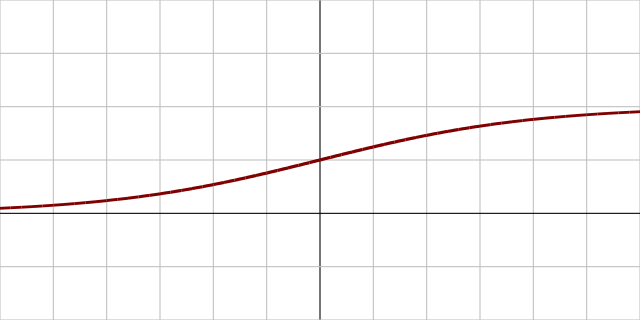
\includegraphics[width=0.7\linewidth]{images/Activation_logistic.png}
\caption{Sigmoid function}
\label{fig:sigmoid}
\end{subfigure}%
\begin{subfigure}{.5\textwidth}
\centering
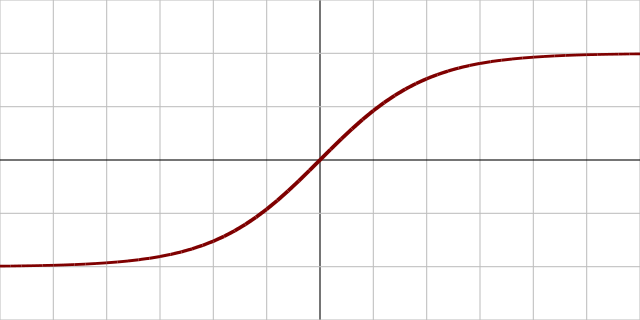
\includegraphics[width=0.7\linewidth]{images/Activation_tanh.png}
\caption{TanH function}
\label{fig:tanh}
\end{subfigure}
\begin{subfigure}{.5\textwidth}
\centering
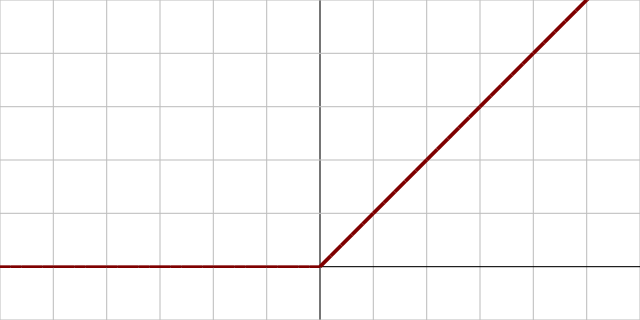
\includegraphics[width=0.7\linewidth]{images/Activation_rectified_linear.png}
\caption{ReLU function}
\label{fig:relu}
\end{subfigure}%
\begin{subfigure}{.5\textwidth}
\centering
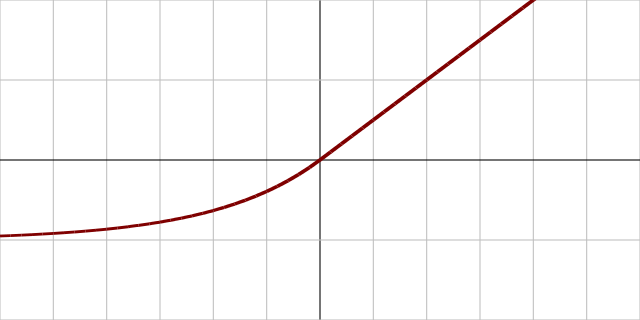
\includegraphics[width=0.7\linewidth]{images/Activation_elu.png}
\caption{ELU function}
\label{fig:elu}
\end{subfigure}%

\caption{Activation functions}
\end{figure}


\subsubsection{Cost Function}
In order to  improve the neural network  there must be an objective measurement of how good or bad the network performs. This is captured with a cost function. If the networks output is close to the desired output, the cost is low, otherwise it is high. A commonly used cost function is mean square error as shown in equation \ref{eq:cost}. 

\begin{equation}
\label{eq:cost}
C =\frac{1}{2}(f(x)-y)^2
\end{equation}

Another commonly used cost function is cross entropy which has significant practical advantages as better local optimums can be found when weights are randomly initialized \cite{golik2013cross, kline2005revisiting}. Using cross entropy cost function instead of mean square error together with the softmax activation function leads to more accurate results \cite{dunne1997pairing}.

\begin{equation}
\label{eq:cross_entropy}
C = -\sum_{c}y_c\log{f(x)_c}+(1-y_c)\log{(1-f(x)_c)}
\end{equation}

\subsubsection{Learning}
The network learns by calculating the cost function and updating its weights in order to minimize the cost function. The learning process is thus an optimization problem.  The cost function is a function of the weights. In order to minimize it gradient descent is used. Gradient descent  calculates the gradient of the cost function with respect to to the weights. It then updates the weights in the opposite direction as to make the cost smaller as seen in \ref{eq:weight_update_derivative}. How big the weight differences are is  decided by the learning rate. In practice gradient descent is not feasible with large amounts of data so instead stochastic gradient descent is used where only a small subset of the training data is used to calculate an estimate of the cost function which makes the training time faster \cite{michaelnielsen2015}. 

\begin{equation}
\label{eq:weight_update_derivative}
w_i= w_i-\lambda\frac{\partial{C}}{\partial{w_i}}
\end{equation}

\subsubsection{Hyper Parameters}
When a neural network is trained it learns what weights it should have. Parameters that affect the training such as how the network architecture but are not learned during training are called hyperparameters. A neural network has a lot of hyperparameters.
\begin{itemize}
\item Learning rate
\item Number of hidden layers
\item Number of hidden nodes
\item Choice of activation function
\item Choice of error measurement
\item Learning rate decay
\item Regularization
\item Initial weights
\end{itemize}
These can be decided by manually testing different combinations. A more rigorous way to choose them is a grid search or random search. In a grid search a finite set of values for each parameter is chosen then all combinations are tried. The one yielding the highest accuracy is selected as the best parameter combination. A random search selects parameters randomly which has shown to be more efficient than grid search \cite{bergstra2012random}. Genetic algorithms breeding new combinations  by combining previous successful combinations can also be applied. A novel approach based on reinforcement learning for generating architectures using the validation accuracy  on the validation set as feedback has been demonstrated to be capable of generating architectures  that rivals the best human-invented architectures on the CIFAR-10 dataset \cite{DBLP:journals/corr/ZophL16}.

\subsection{Convolutional Neural Network}

Convolutional neural networks (CNN) have dramatically improved object recognition and is the current state-of-the-art for this task \cite{szegedy2015going}. In a CNN  each neuron is connected in overlapping tiles giving  the network  locality in a two-dimensional space. This works well for input data that can be treated as images or grids \cite{szegedy2015going}.

\subsubsection{Input}
Instead of treating input data as a 1-dimensional vector it is treated as  3-dimensional vector. An  rgb image of size $9\times9$ would have dimensions  $9\times9\times3$ since it has 3 color channels. 

\subsubsection{Patch Size}
The patch size determines how large area a neuron covers. A $3\times3$ patch is the most common size and means that each neuron in layer $i+1$ is connected to a  $3\times3$ tile of neurons in layer $i$.

\subsubsection{Stride}
The stride determines the distance between each input to the filter.

\subsubsection{Filter}
The number of filters determines how many features can be detected in each layer since the filters share weights.

\subsubsection{Pooling}
Pooling means reducing the dimensions of the input by summarizing its inputs. A $2\times2$ max pooling for example would take an input of $2\times2$ and output $1\times1$ with the highest value found in the input and stride over data.

\section{Candy Crush Saga}
Candy Crush Saga (Candy) is a popular match-three game released on Facebook in 2012  and  later on multiple platforms. The game has grown to be complex due to continuously adding new features during the development of more than 2000 levels.  We therefore will not provide a complete description of the game and instead refer the reader to the Candy Crush wiki available online.\footnote{http://candycrush.wikia.com} We will describe the basics interesting for the thesis.

\subsection{Basic Game Play}
The basic game play consists of swapping  horizontally  or vertically adjacent tiles on a 9x9 game board such that a pattern of three or more candies of the same color are in a horizontal or vertical line. This is why it is called a match-three game. There are 144 possible unique swaps, 72 vertical and 72 horizontal, if direction is ignored.


The matched candies are removed from the game board  and if more than three candies are matched special candies are created as shown in Fig \ref{fig:special_candies_swap}. Special candies are more powerful than normal candies as they do not only remove themselves when matched but also other candies. Making special candies is therefore an important part of the game strategy. There is also multiple types of blockers  such as frostings  that can be residing on a tile making it impossible to match with the candy underneath until the frosting has been cleared.

Solving the game is NP-hard \cite{DBLP:journals/corr/Walsh14}. The state space differs between levels but is large, an experiment showed that the state space on level 13 is approximately $10^{182}$ \cite{poromaa2016}.


\subsection{Game Modes}
There are five different kinds of levels with different objectives.

\begin{itemize}
\item \textbf{Timed levels} – Achieve a certain score before time runs out 
\item \textbf{Score levels} – Achieve a certain score within a fixed number of moves  as shown in Fig \ref{fig:candy_crush}
\item \textbf{Order levels} – Clear all orders within a fixed number of moves, an order could be clear 90 red candies
\item \textbf{Mixed levels} – Complete a combination of other objectives 
\item \textbf{Ingredients levels} – Clear all ingredients within a fixed number of moves
\item \textbf{Jelly levels} – Clear all jellies within a fixed number of moves
\end{itemize}
Having multiple game modes requiring different strategies makes the game more challenging for AI.


\begin{figure}
\centering
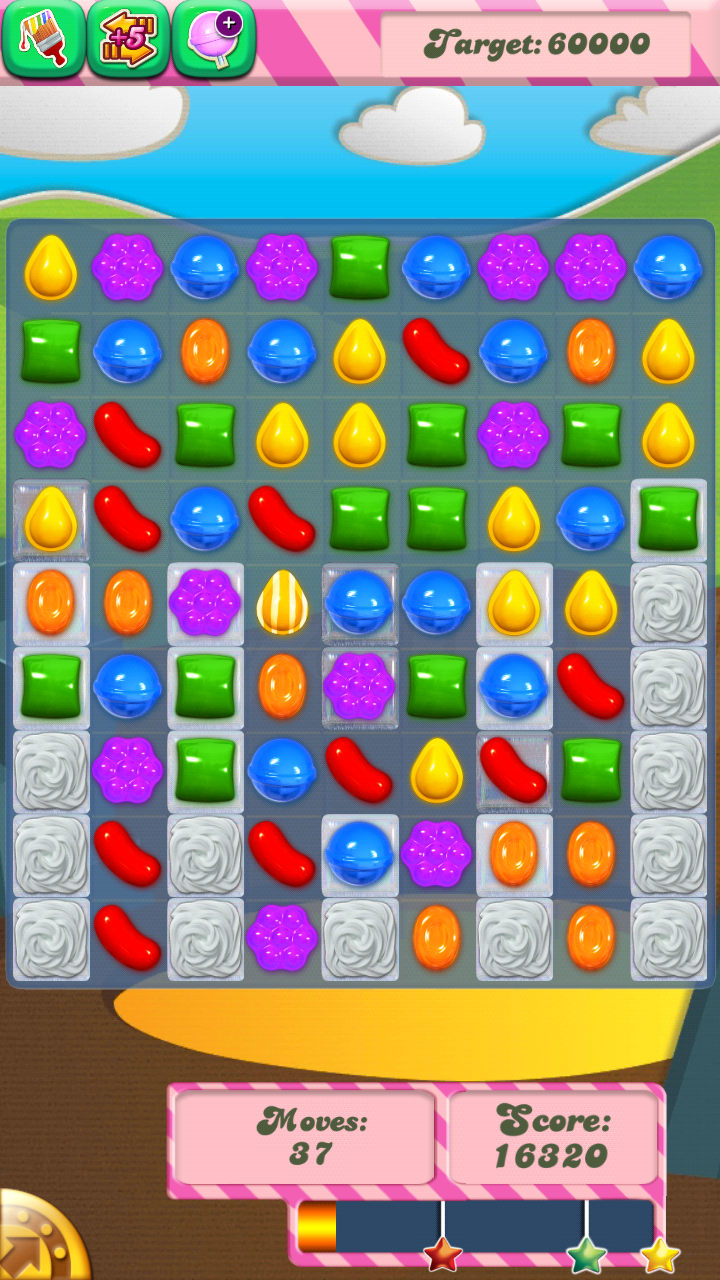
\includegraphics[width=0.8\textwidth]{images/candy_crush.png}
\caption{A score level, the user has 37 moves left to achieve the target score of 60000}
\label{fig:candy_crush}
\end{figure}


\begin{figure}
\centering
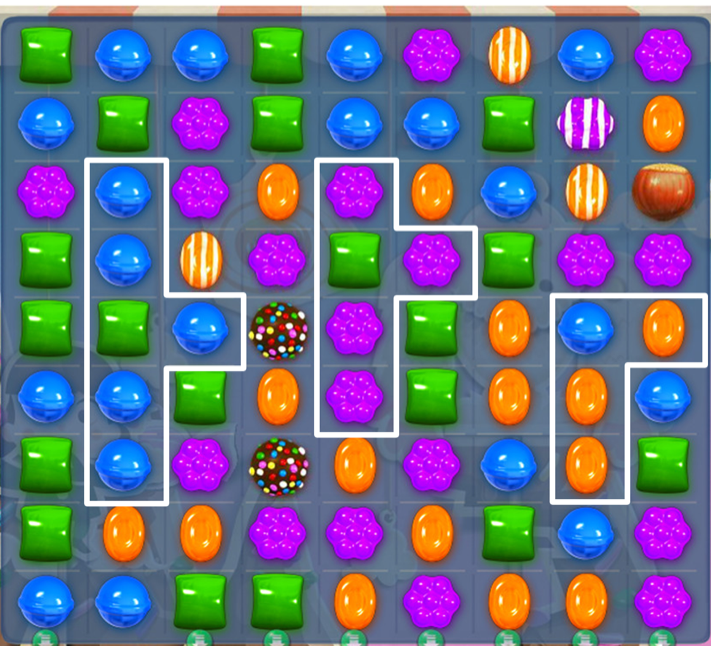
\includegraphics[width=0.8\textwidth]{images/special_candies_swap.png}
\caption{Three different swaps, the leftmost creates a color bomb, the center creates a horizontal striped candy, the rightmost creates no special candy}
\label{fig:special_candies_swap}
\end{figure}

\chapter{Method}
In this chapter we give a detailed description of our method. It is divided into two parts, experiments on a simplified version of Candy and experiments on Candy.

\section{Simplified Candy}
When the  thesis started we did not yet have training data available from Candy and we wanted to  explore deep learning on a simplified problem  to get a notion of how powerful and suitable it is for our space of problems. Therefore we decided to:
\begin{enumerate}
\item Build a simplified version of Candy
\item Create a deterministic greedy bot
\item Generate dataset from the greedy bot playing Candy
\item Train a DNN
\item Evaluate classification performance
\end{enumerate}

Since we do not have any human difficulty data for simplified Candy we do not attempt at predicting difficulty for this experiment. We only explore the classification task.

\subsection{Simplified Candy}
Simplified Candy was implemented in C++ and can be played with or without a GUI. It can be seen in Fig. \ref{fig:candy_small}. It has a slightly smaller game board of $8\times8$ compared to the real game which has $9\times9$. It has 5 different candy colors instead of 6. It has no special candies or blockers. It has no objectives. The game automatically stops after a 60 seconds and the score increases  proportionally to the number of candies cleared. New candies are generated randomly from a uniform distribution. 
\begin{figure}
\centering
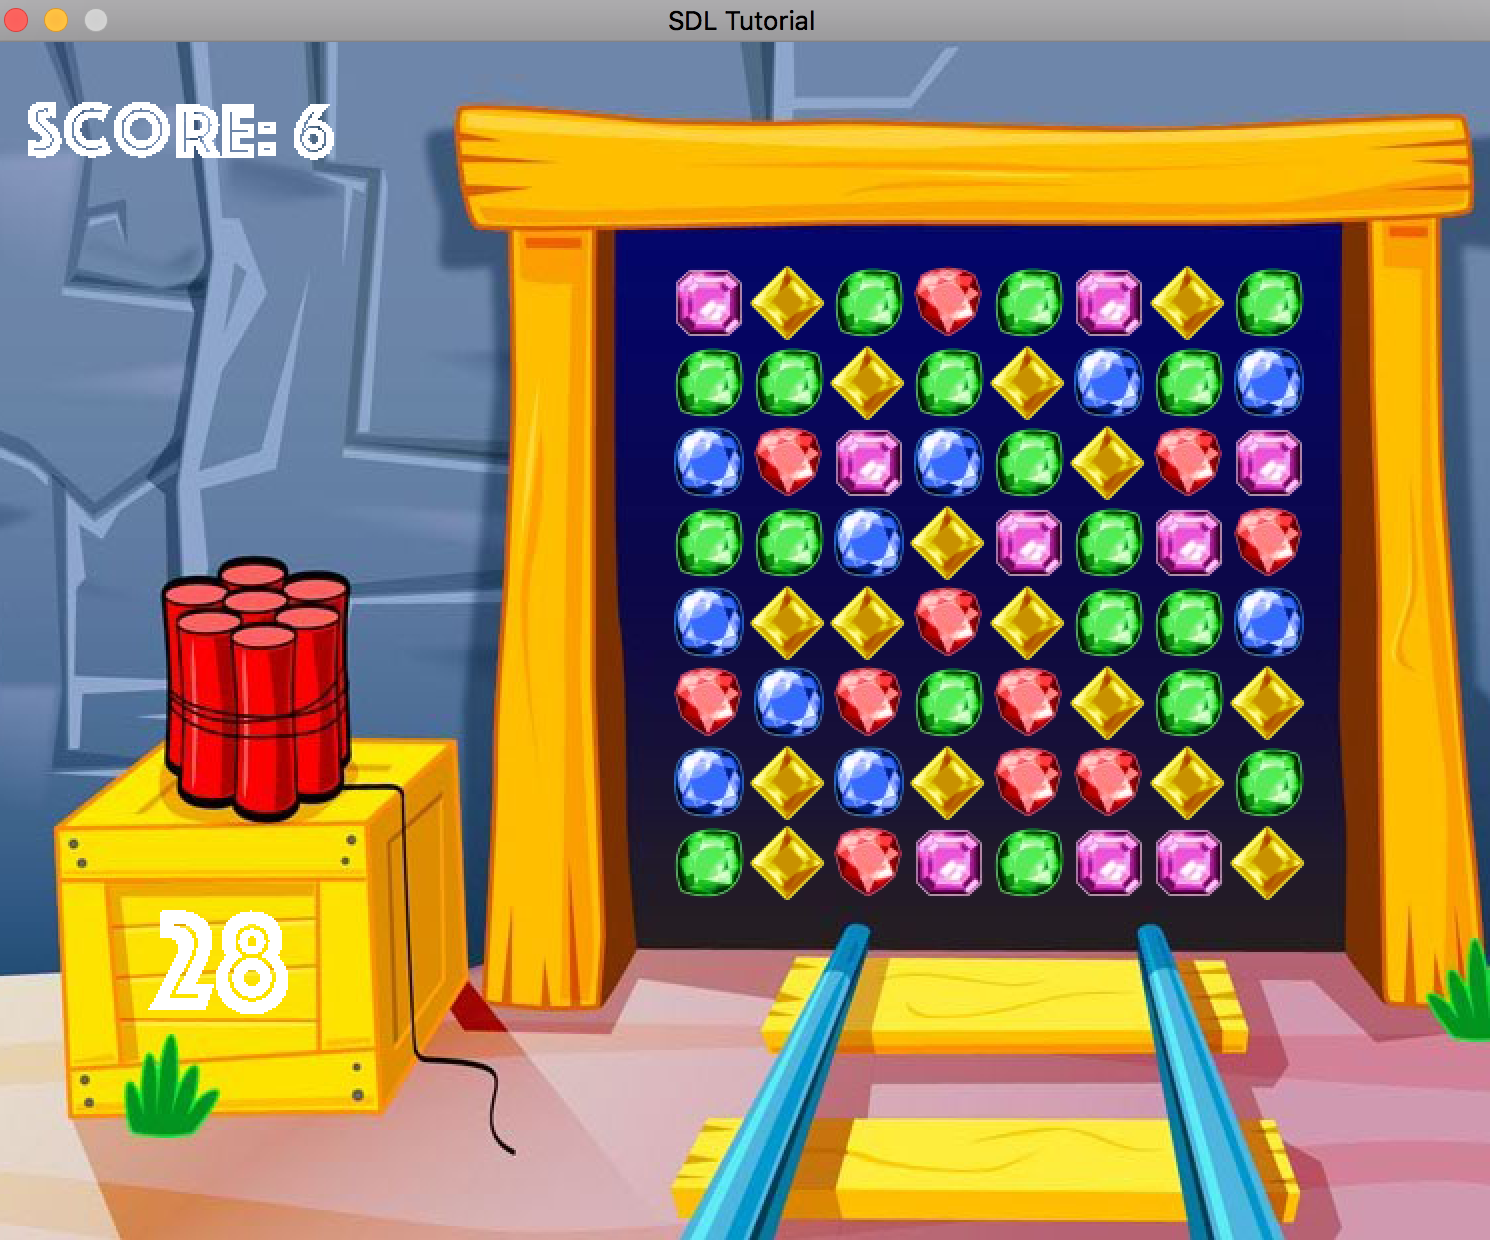
\includegraphics[width=\textwidth]{images/candy_small.png}
\caption{Simplified Candy}
\label{fig:candy_small}
\end{figure}

\subsection{Deterministic Greedy Bot}
We created a deterministic greedy bot that always selects the move which clears the most candies. It will always prefer a five-match to a four-match and a four-match to a three-match. If there are multiple moves that clears equally many candies, it prefers horizontal swaps to vertical swaps  and north-west positions to south-east positions. This makes the bot deterministic and it is possible to calculate what move it will select from any game board. This is important as  the data becomes 100\% predictable which means that a machine learner can get 100\% validation accuracy. When learning from non-deterministic strategy it is not possible and you do not know what the theoretical maximum validation accuracy is.

\subsection{Generate Dataset}
We generated a dataset from the deterministic greedy bot playing simplified Candy. It has only two feature planes, one for colors and one for valid moves. Each color is encoded $0 \leq c\leq 4$. The valid move feature plane is binary and encodes for each position whether it can be part of  a valid move. If two positions are adjacent and both have a 1 in the valid move feature plane they constitute a valid move.
\\

\begin{figure}[!tbp]
  \centering
  \begin{minipage}[b]{0.4\textwidth}
\begin{tabular}{|l|l|l|l|l|l|l|l|}
\hline
2&0&1&4&3&0&0&1\\
\hline
1&4&0&3&2&2&3&4\\
\hline
4&1&2&2&3&1&4&1\\ 
\hline
1&3&0&1&4&2&0&3\\
\hline
1&0&3&0&1&3&1&3\\ 
\hline
2&2&4&0&4&1&1&4\\
\hline
4&3&0&3&0&4&2&1\\ 
\hline
2&1&1&4&1&2&4&4\\
\hline
\end{tabular}
    \caption{An example color plane, the numbers denotes different colors\\}
  \end{minipage}
  \hfill
  \begin{minipage}[b]{0.4\textwidth}
\begin{tabular}{|l|l|l|l|l|l|l|l|}
\hline
0& 0& 0& 0& 0& 0& 0& 0\\
\hline
1& 0& 0& 1& 1& 0& 0& 0 \\
\hline
1& 1& 0& 1& 1& 0& 0& 0\\
\hline
0& 0& 1& 1& 0& 0& 0& 0 \\
\hline
0& 0& 1& 0& 1& 1& 0& 0 \\
\hline
0& 0& 0& 1& 1& 1& 0& 1 \\
\hline
0& 0& 1& 1& 1& 1& 1& 1 \\
\hline
0& 0& 0& 1& 1& 1& 0& 0 \\
\hline
\end{tabular}
    \caption{The corresponding valid move feature plane}
  \end{minipage}
\end{figure}


There are $board\_size * (board\_size-1)$ horizontal swaps since there are $board\_size$ number of rows and on each row there are $board\_size-1$ horizontal swaps if we ignore the direction of the swap. Since there are as many horizontal swaps as vertical swaps the total number of swaps are $2*board\_size*(board\_size-1)$. For this particular dataset $board\_size=8$ so there are $2*8*7=112$ different swaps. A move is therefore encoded as a number between $0\leq n \leq 111$ as seen in Fig \ref{fig:simple_move_encoding}. 

\begin{figure}[]
\centering
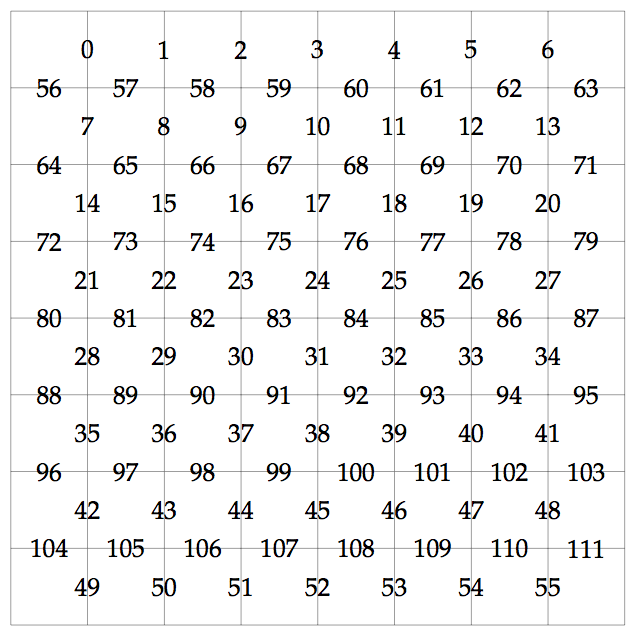
\includegraphics[width=0.7\textwidth]{images/encoding_small_moves.png}
\caption{Encoding of moves}
\label{fig:simple_move_encoding}
\end{figure}

The dataset is stored as a CSV-file. Each line corresponds to a datapoint. The first $2*8*8=128$ numbers are the features consisting of the two feature planes for each of the 64 game board positions, and the last number is the move.

\subsection{Neural Network Architecture}
The network architecture was decided by manual experimentation. We would have liked to perform a grid search on many combinations of parameters but we deemed that to be too time consuming and computationally expensive to be viable for this work. \\

\begin{tabular}{ l | r }
Learning rate & 0.05 \\
Batch size & 128 \\
Patch size & 3 \\
Stride & 1 \\
Filters & 34 \\
Pooling & None \\
Padding & Same \\
Convolutional layers & 3 \\
Fully-connected layers & 1 \\
Hidden nodes & 256 \\
Activation function & ReLU \\
Error measurement & Cross entropy \\
Learning rate decay & 0.96 \\
Regularization & None \\
Initial weights & 0.1 \\
\end{tabular}

We chose to use a convolutional neural network since our game board has a grid structure and it has had great performance on other board games such as Go \cite{alphaGo2016}. Since generating data from the MCTS bot took a long time we had a smaller dataset while tuning the hyperparameters than what we used for final evaluation. We tested different number of convolutional layers and found that more than three layers do not improve validation accuracy and increases overfitting. Pooling which reduces the dimensions of the input is often used in image recognition where the images for example can have the size 256x256. We chose not to use pooling since our 9x9 game board already is small.

\subsection{Neural Network Evaluation}
The dataset was divided into a training set and a validation set. The training set is used during training to update the weights of the network. The validation set is used for evaluation. The performance measured used during training is validation accuracy as seen in equation \ref{eq:validation_accuracy}.  We also calculated validation top 2 accuracy and validation top 3 accuracy meaning how often the correct move was found in the top 2 and top 3 moves.

\begin{equation}
\label{eq:validation_accuracy}
\frac{correct}{total}
\end{equation}

The validation accuracy is not a perfect measurement of game strategy since the selected action in a game state is non-deterministic, meaning that a player in  certain game state multiple times may choose different actions. If a player is in a state with 10 legal actions and the player selects one out of two actions with 50\% probability then the theoretical maximum validation accuracy would be 50\%, but if the network learned the correct probability distribution it would have perfectly learned the game strategy. The ideal would be to use a measurement between the distance of the real and predicted probability distributions rather than validation accuracy such as the Kullback–Leibler divergence shown in equation \ref{eq:kullback_leibler_divergence}.

\begin{equation}
\label{eq:kullback_leibler_divergence}
\sum_i P(i)\ln\frac{P(i)}{Q(i)}
\end{equation}

However, since the state space is so large it is very rare that there are multiple training samples from a specific state making it impossible to estimate a probability distribution in the specific state. Validation accuracy is therefore chosen for pragmatic reasons.

Having no other benchmarks this  is compared to the expected accuracy of randomly selecting moves in each game state calculated as shown in equation \ref{eq:random_accuracy} where $S_{i}$ is the number of moves available in state $i$.

\begin{equation}
\label{eq:random_accuracy}
\frac{1}{n}\sum_i^n\frac{1}{S_{i}}
\end{equation}

\section{Candy}
The experiment on Candy consists of the following steps.
\begin{enumerate}
\item Generate dataset from an MCTS bot playing Candy
\item Train a DNN
\item Play different Candy levels with different bots using DNN and MCTS
\item Evaluate performance measured as cumulative success rate and mean success rate
\item Create a regression models to predict human difficulty from bot difficulty measured as attempts per success
\end{enumerate}

Just as for simplified Candy we generate training data and then train a neural network but then we proceed to use the neural network to actually play the game and measure the bots performance in terms of success rate and create a model to predict human difficulty from bot difficulty measured as attempts per success.

\subsection{Monte Carlo Tree Search}
MCTS algorithm used was provided by King. It is written in C++ on top of the Candy source code. The implementation has a few novelties. Instead of only using win or loss as the signal a  continuous signal is used based on partial goals such as the number of jellies cleared and/or the score.  We treat it as a black box that can be configured to use a trained DNN during playouts hence a more detailed description is not necessary but is available in Erik Poromaas master thesis \cite{poromaa2016}.

\subsection{Generate Dataset}
Since we want to use the neural network to predict difficulty for players it would make most sense to use game play data from players. However, that data was not available and we could not get it for the thesis. We did have an MCTS bot that could play the game very well. We let the MCTS bot using 1000 simulations per move play a diverse set of levels between level 1000 and level 2000 and added logging of all $(state, action)$ pairs  during game play in a CSV-format directly usable for training a neural network. We gathered close to 2 million data points. 50k data points was used for validation and the rest was used for training.

\subsubsection{Data Representation}
The feature planes are:

\begin{multicols}{2}
\begin{enumerate}
\label{tab:feature_planes}
\item HORIZONTAL MOVES AVAILABLE
\item VERTICAL MOVES AVAILABLE
\item MISSING TILES
\item CANDY COLOR RANDOM
\item CANDY COLOR NONE
\item CANDY BLUE
\item CANDY GREEN
\item CANDY ORANGE
\item CANDY PURPLE
\item CANDY RED
\item CANDY YELLOW
\item NUM CANDY COLORS
\item JELLY
\item BLOCKERS
\item LOCKS
\item BOARD ITEM TYPE NORMAL
\item BOARD ITEM TYPE ROW
\item BOARD ITEM TYPE COLUMN
\item BOARD ITEM TYPE WRAP
\item BOARD ITEM TYPE HOT
\item BOARD ITEM TYPE BOMB
\item BOARD ITEM TYPE SWEDISH FISH
\item BOARD ITEM TYPE INGREDIENT CHERRY
\item BOARD ITEM TYPE INGREDIENT HAZELNUT
\item BOARD ITEM TYPE TIME REFILL
\item BOARD ITEM TYPE PEPPER CANDY
\item BOARD ITEM TYPE LICORICE BLOCKER
\item BOARD ITEM TYPE COCONUT WHEEL
\item BOARD ITEM TYPE JOKER
\item BOARD ITEM TYPE MYSTERY CANDY
\item BOARD ITEM TYPE CHAMELEON CANDY
\item BOARD ITEM TYPE FROG
\item BOARD ITEM TYPE MULOCK KEY
\item BOARD ITEM TYPE UFO
\item NUM BOARD ITEM TYPES
\item NUM MOVES LEFT
\end{enumerate}
\end{multicols}

Colors are encoded as separate binary feature planes compared to the simplified dataset  where there was only one color feature plane and different colors used different numbers. This makes more sense as the color only has categorical meaning. The valid moves feature plane was split up in one for horizontal moves and one for vertical moves. This makes no difference as the neural network manages to learn both representations. Moves are encoded as in the first experiment as well except for that the larger game board makes it a number $0\leq n \leq 143$ instead of  $0\leq n \leq 111$ as seen in Fig \ref{fig:move_encoding}.  

\begin{figure}[]
\centering
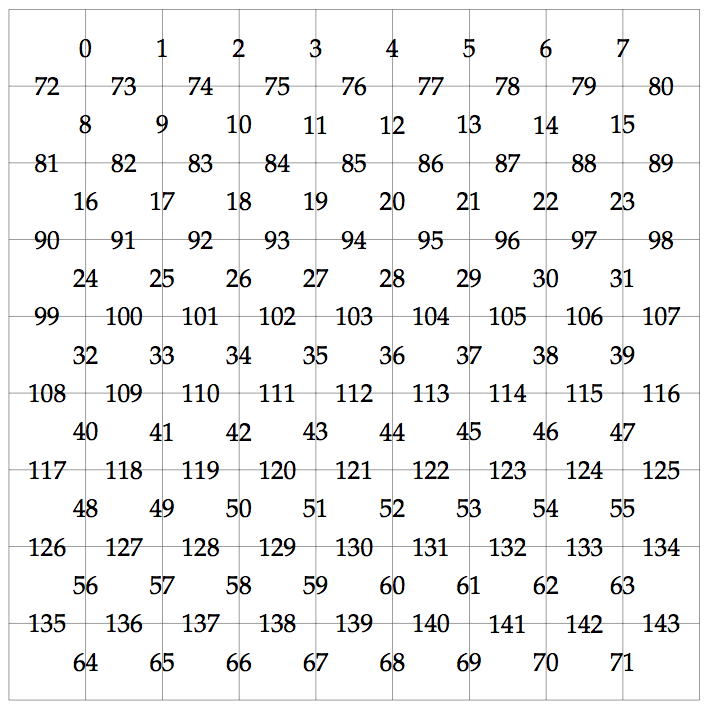
\includegraphics[width=0.7\textwidth]{images/encoding_big_moves.png}
\caption{Encoding of moves}
\label{fig:move_encoding}
\end{figure}

\subsubsection{Drawbacks}
While direction of the move does not matter in the simplified Candy, it does matter in Candy. When matching two special candies the impact on the game board will be different depending on direction. In order to capture this we would need to distinguish between 288 moves instead of 144. This may make it impossible to learn advanced strategies where certain combinations of special candies and directions are necessary to clear the level. However, we do note that we have a 50\% chance of making the swap in the best direction  and that having two adjacent striped candies is not a common situation so we decided to discard the direction as having twice as many classes would make it harder to train the DNN.

There are a few other drawbacks with the dataset.  The biggest one is that there is no feature plane for the goal of the level. If the goal is clearing jellies the data does not contain the number of jellies to be cleared or if the goal is to clear ingredients there is no feature plane containing the number ingredients left to be cleared. This will likely make it harder for the network to learn to prioritize the goal when the number of moves left are few rather than creating fancy special candies. 

\begin{figure}
\centering
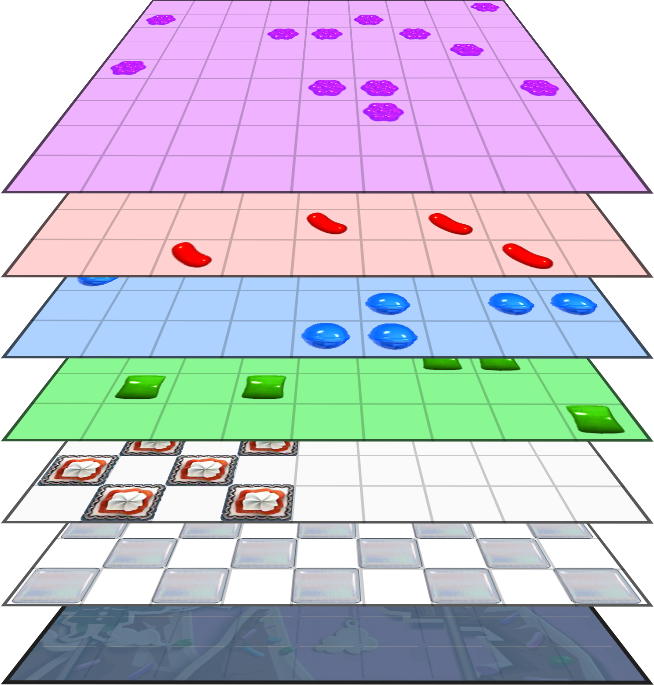
\includegraphics[width=0.7\textwidth]{images/game_board_feature_planes.png}
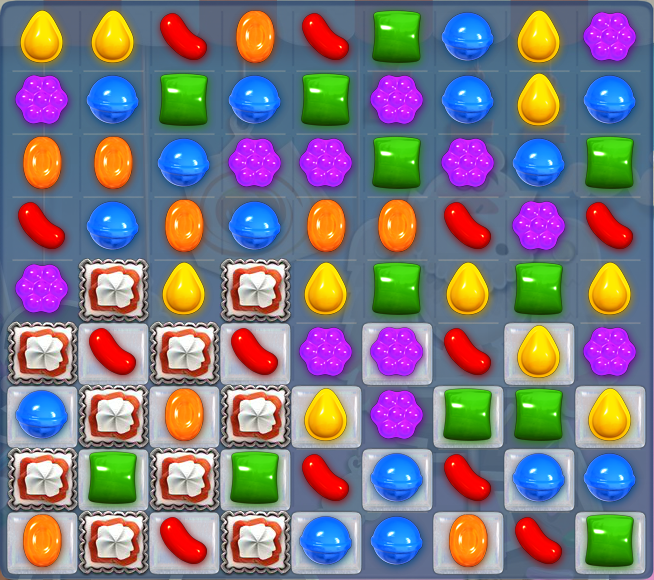
\includegraphics[width=0.7\textwidth]{images/game_board.png}

\label{fig:game_board}
\caption{Example game board and its feature planes}
\end{figure}

\subsection{DNN Architecture}
We used the same DNN as for Simple candy.

\subsection{Using DNN}
The DNN was used through an HTTP server written in Python because we deemed it to cumbersome to embed it inside the MCTS C++ source code using the immature TensorFlow C++ API. Having the HTTP server running on the same physical machine as the bot made the networking overhead  insignificant.

We tested  to let the DNN play by itself and during MCTS playouts. The highest probable move according to the DNN was selected.

\subsection{Neural Network Evaluation}
Training is evaluated the same as for simple Candy. We used in total 4 bots for comparisons. The bots are also compared to human players. We compare the cumulative success rates of the bots to measure their performance. We also fit models to predict human attempts per success from the bots attempts per success in order to measure their predictive power. MCTS performs 100 attempts per level and DNN performs both 100 and 1000 attempts per level because it is much faster. 

\subsubsection{Random Bot}
The random bot selects moves randomly from a uniform distribution. It is the default baseline. 

\subsubsection{DNN Bot}
The DNN bot selects the most probable move according to the deep neural network. It does not do any search. 

\subsubsection{MCTS + Random Bot}
The MCTS + Random  bot uses MCTS with random playouts. It serves as a baseline for MCTS + DNN bot.

\subsubsection{MCTS + DNN Bot}
The MCTS + DNN bot uses MCTS with DNN during playouts where the highest probable move according to the DNN was selected.

\subsection{Prediction Models}
We played 361 levels with the bots to calculate the bot difficulty measured as attempts per success. We let each bot play make 100 attempts on each level except for the DNN which we allowed to make 1000 attempts because it is much faster. Player data was available for those levels so we could also calculate human attempts per success. Bot difficulty is not the same as human difficulty but they are correlated. We fit a regression model to predict human attempts per success from bots attempts per success. We use mean absolute error as a measure of predictive accuracy which intuitively means how wrong the predictions were on average.

We divide the levels into three groups, green, yellow and red depending on how hard they are for each because we saw that the relationship between human attempts per success and bot attempts per success differed for easier levels and harder levels. We fit a separate prediction model for each group for each bot. The green levels have an attempts per success lower than or equal to a preselected cutoff which was 20 for MCTS and 200 for DNN. The yellow levels  have a higher attempts per success than the cutoff. Red levels have zero successes so attempts per success is undefined. We used the mean of human attempts per success as predicted value for red levels. We also use 5 as a minimum value for predicted attempts per success because levels are not easier than that for humans.

\section{Software}
We used the deep learning library TensorFlow to implement the DNN. Google created TensorFlow to replace DistBelief which is widely used within Google \cite{abadi2016tensorflow}. TensorFlow is written in C++ with an API available in Python. It is not as fast as other deep learning libraries available such as Torch and Theano \cite{bahrampour2015comparative}, but comes with many helpful tools. TensorBoard is a web interface that visualizes training. When creating a TensorFlow graph it is possible to add nodes for logging measurements such as validation accuracy, cross entropy and learning rate. TensorBoard can display the logged measurements in graphs  dynamically created during training as seen in Fig. \ref{fig:tensorboard}. 

\begin{figure}
\centering
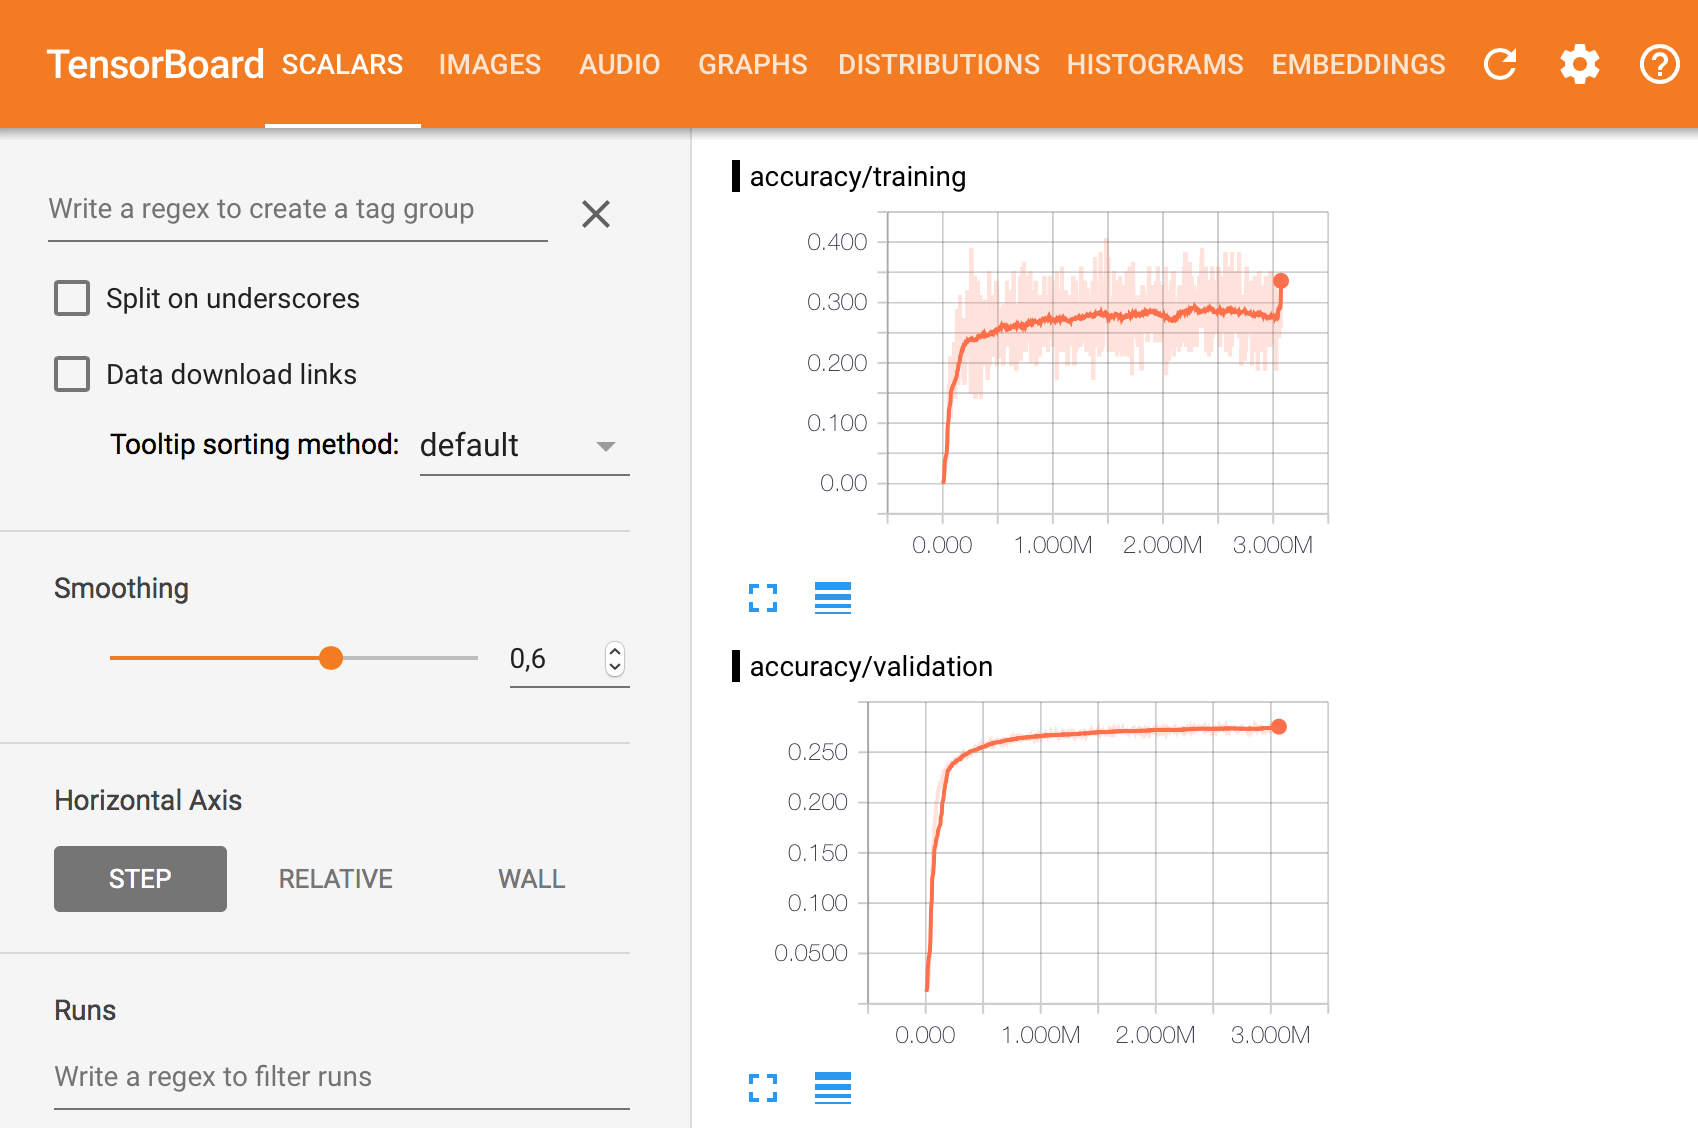
\includegraphics[width=\textwidth]{images/tensorboard.png}
\caption{TensorBoard}
\label{fig:tensorboard}
\end{figure}

\section{Hardware}
We used a g2.8xlarge GPU server from Amazon Web Services for training neural networks.
It has:
\begin{itemize}
\item  4 GPU
\item 32 vCPU
\item 60 GiB memory
\item  2x120 SSD storage
\end{itemize}

The game play ran on virtual machines with unknown specifications.




\chapter{Results}

\section{Training Neural Networks}
This part shows the performance of the DNN during training. The validation accuracy shows how the DNN is expected to perform on unseen data. We also included how often the correct move was in the top 2 and top 3.

\begin{figure}[!htb]
\centering
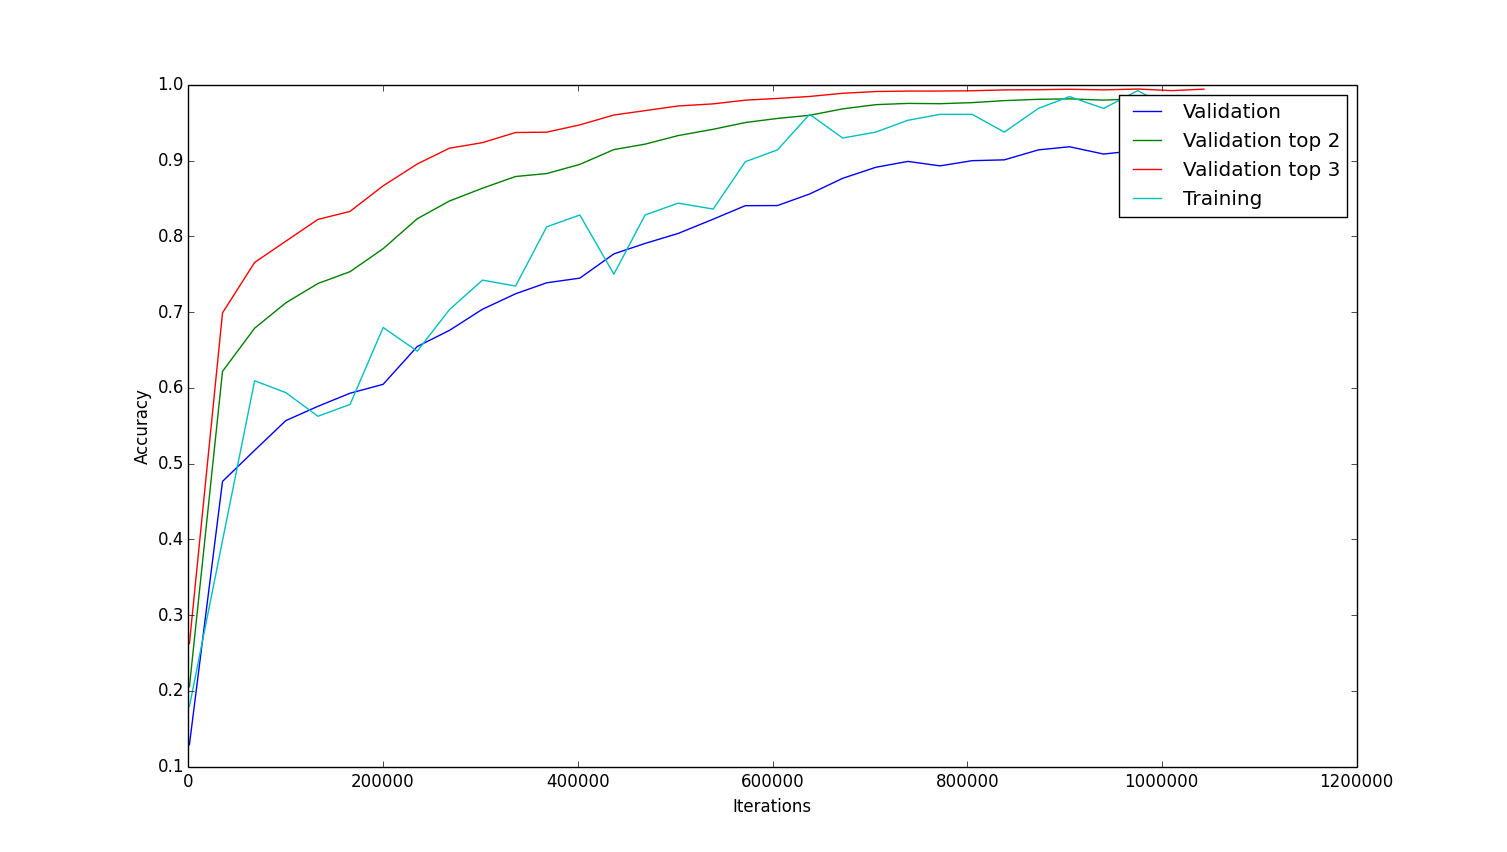
\includegraphics[width=\textwidth]{images/candy_small_validation.png}
\caption{Validation accuracies on simplified Candy. Validation top 2 means how often the correct move was one of the top 2 predicted ones, validation top 3 means how often the correct move was one of the top 3 predicted ones.}
\label{fig:candy_small_validation_accuracy}
\end{figure}

\begin{table}
\caption{Simplified Candy result. Random accuracy is the expected validation accuracy when selecting randomly from the available moves in each game state.}
\centering
\begin{tabular}{ l | r }
\hline
Training size & 450 176\\
Validation size & 26 000\\
Average number of moves per state & 23.2 \\
Random accuracy & 4.9\% \\
Validation accuracy & 92.2\% \\
Validation top-2 accuracy & 98.3\% \\
Validation top-3 accuracy & 99.4\% \\
Training accuracy & 98.9\% \\
Iterations & 18k \\
Duration & 69h \\
\hline
\end{tabular}
\end{table}

\begin{figure}[!htb]
\centering
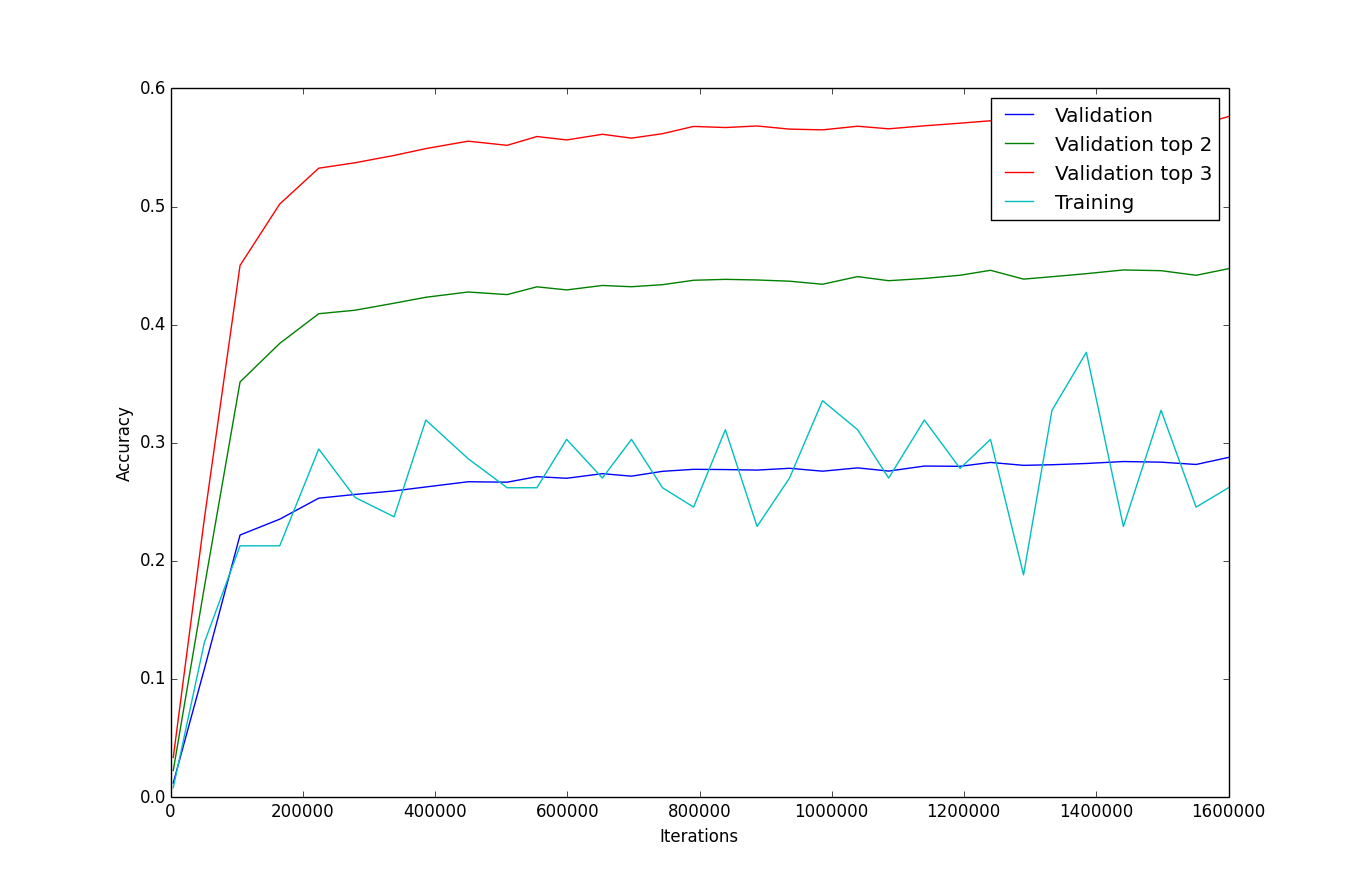
\includegraphics[width=\textwidth]{images/real_validation.png}
\caption{Validation accuracies on Candy. Validation top 2 means how often the correct move was one of the top 2 predicted ones, validation top 3 means how often the correct move was one of the top 3 predicted ones.}\label{fig:candy_real_validation_accuracy}
\end{figure}

\begin{table}
\caption{Real data}
\centering
\begin{tabular}{ l | r }
\hline
Training size & 1 594 714\\
Validation size & 50 000\\
Average number of moves per state & 13.4 \\
Random accuracy & 16.7\% \\
Validation accuracy & 28.3\% \\
Validation top-2 accuracy & 44.4\% \\
Validation top-3 accuracy & 57.3\% \\
Training accuracy & 30.4\% \\
Iterations & 1 000 000 \\
Duration & 7 days \\
\hline
\end{tabular}
\end{table}

\section{Bot Performance}
We compare the strength of the bots using mean success rate on all levels shown in Table \ref{tab:success_rate}. In Fig \ref{fig:cumulative_sr} the cumulative success rate over levels is shown, the higher the better.

\begin{figure}[!htb]
\centering
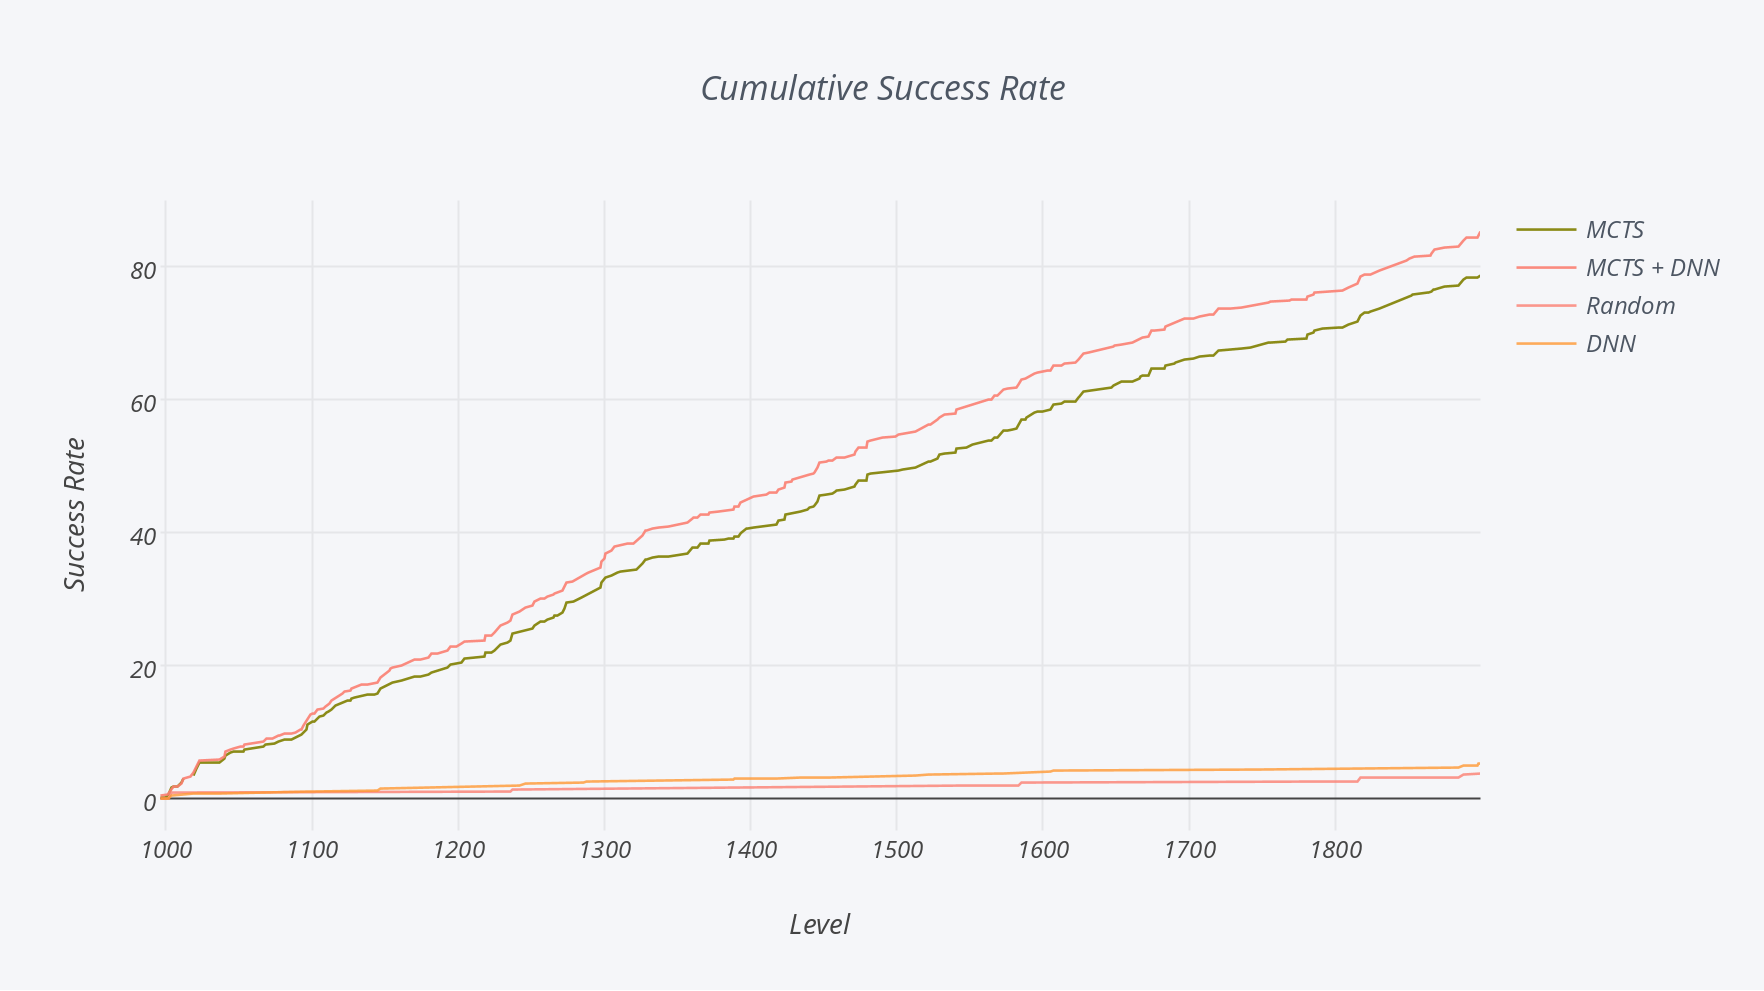
\includegraphics[width=\textwidth]{images/cumulative_sr.png}
\caption{Cumulative success rate for each method}
\label{fig:cumulative_sr}
\end{figure}

\begin{table}
\caption{Success rate for each method}
\centering
\begin{tabular}{l{c}r}
\hline\hline
Method & Mean & Standard deviation \\
\hline
MCTS + Random & 0.212663 & 0.226270 \\
MCTS + DNN & 0.229924 & 0.230549 \\
Random & 0.010199 & 0.066933 \\
DNN & 0.014281 & 0.046330 \\
\hline
\end{tabular}
\label{tab:success_rate}
\end{table}

\section{Difficulty Predictions}
Table \ref{tab:prediction_accuracy} shows the mean absolute errors on 361 levels for each bots. It shows how well the model could predict human difficulty from the bots difficulty. 

\begin{table}
\caption{Accuracy of predicted attempts per success for each bot}
\centering
\begin{tabular}{l{c}cr}
\hline\hline
Method & Attempts & Mean absolute error & Standard deviation\\ 
\hline
MCTS & 100 & 3.02 & 4.12	 \\
MCTS + DNN & 100 & 2.96 & 4.06	 \\
DNN & 100 & 3.28  & 4.41 \\
DNN & 1000 & 2.85  & 3.85 \\
\hline
\end{tabular}
\label{tab:prediction_accuracy}
\end{table} 
 
\chapter{Discussion}
\section{DNN Training}
The validation accuracy on the simplified dataset is high and reaches 92.2\% as seen in Fig. \ref{fig:candy_small_validation_accuracy}. Given more data, more training time and a bigger model  it would likely be able to become even better. Perhaps close to 100\%.

The validation accuracy on the MCTS data is much lower at 28.3\% as seen in Fig. \ref{fig:candy_real_validation_accuracy}. This is not surprising as  it is generated from a non-deterministic algorithm. 28.3\% is still a lot higher than 16.3\% which random guessing would give. Given that we do not know how predictable the MCTS data is it is hard to know how good our network has been on learning it. It could be that 30\% is the theoretical maximum validation accuracy, in which case 28.3\% is good, or it could be much higher, in which case 28.3\% might be pretty bad. 

The training accuracy jumps up and down a lot in the  graphs. That is because  it is calculated on a small randomly selected batch  of 128 datapoints. The training accuracy appears to be close to the validation accuracy for both datasets. This  implies that the neural network has not overfitted which suggests that there is room for increasing the model size. We would have done that but ran out of time.  During the thesis work we continuously collected  more data and the DNN overfitted until the last dataset which was  large enough to make it not overfit. 

Looking at validation, validation top-2 and validation top-3 accuracies we note that the DNN trained on MCTS data improves from 28.3\% to 44.4\% to 57.3\%. This implies that even when it fails to select the correct move the correct move is often in the top-3. Considering that there are many situations in Candy where multiple moves appear to be equally good it is not surprising if it is hard to distinguish between them. 

\section{MCTS}
Playing without any search, DNN outperforms random and it improves MCTS when used during playouts as can be seen in Fig. \ref{fig:cumulative_sr}. This demonstrates  that the DNN has learned useful knowledge of the game from the data. It is interesting to note how much worse pure DNN performs compared to pure MCTS as others have succeeded in making DNNs as strong as MCTS in Go. The results in Go have been achieved with expert moves while we used data from an MCTS bot weaker than expert players. One of the problems with the training data is that it does not include the goals of the game. For this reason alone it is going to be difficult to perform well without any search. The improvement between using search or no search is much greater than the improvement between using the DNN or not. The gains from using DNN must outweigh the fact that it takes a lot of work to train it and that it will need to be continuously retrained when new features are added to the game in order for it to be worth continued usage in the future.

\section{Predicting Human Difficulty}
The most surprising result is that even though the DNN is much weaker than MCTS it is about as good or better at predicting human difficulty when it is allowed to make 1000 attempts per level instead of 100 as can be seen in Table \ref{tab:prediction_accuracy}. When the DNN only makes 100 attempts per level it is the worst predictor. Since the DNN is much faster than MCTS this means that comparable estimations of human difficulty can be obtained in minutes instead of hours. This can change the level designers work flow  giving them a much faster feedback loop making more tweaks possible before release.

\section{Future Work}
\subsubsection{Improve Architecture}
As we were heavily restricted by time  we did not investigate the space of possible neural networks very much. There is an almost infinite number of things one could try. If one has time then training a deeper DNN with more data would likely show better results. We did not overfit with our architecture so training a deeper DNN would be the next thing to try.

\subsubsection{Improve Data}
The data we used excluded important information such as the goal of the level. It also did not contain the direction of moves. Using better data would likely show better results.

\subsubsection{Real User Data}
We initially intended to use real user data for this thesis. We spent a lot of time collecting  it for Candy Crush Soda Saga which required adding code to the code base and getting it released.  It was however aborted as there were problems replaying the games outside of our control. It would be interesting to continue this experiment and train on expert players and see what that does for performance.

\subsubsection{Reinforcement Learning}
In this thesis we only attempted to make the neural network learn how someone else plays, in this case a MCTS bot. The performance metric being minimized is how well the neural network can predict how someone else would play. It could be interesting to change the aim to play as good as possible. Using reinforcement learning the DNN weights could be altered after having been trained on a dataset to maximize its performance. Play a level, see how well it performed, update the weights in order to make it play better the next time. 

\subsubsection{Qualitative Exploration of Learning}
We only made quantitative measurements of performance. What kind of moves and strategies does the neural network learn? We have no idea, we only know that it gets a certain validation accuracy and that it gets a certain success rate in a game. Exploring what kind of moves  it learns and does not learn could perhaps give some interesting insights.

\section{Ethics of Artificial Intelligence}
There are two main concerns of Artificial Intelligence (AI). The threat of super intelligence and the economic impact of automation.

\subsubsection{Super Intelligence}
AI can be  divided into three categories  depending on how powerful it is. Today all AI available is in the category artificial narrow intelligence (ANI) which means that it is task specific. DeepBlue is better than any human at chess but playing chess is all it can do. The second category is artificial general intelligence (AGI) and  includes AI that is about as capable as a human, meaning that it is capable of doing general things that humans can do. The third category is  artificial super intelligence (ASI) and  consists of AI superior to human beings. Once AGI is invented, it might be able to recursively improve its software in order to make it more capable and eventually reach ASI \cite{bostrom1998long}. If ASI turns malignant it might send humans to extinction. In this thesis we explore yet another application of ANI which in its current state does not pose an existential threat to humanity.

\subsubsection{Economic Impact}
AI capable of replacing human labor  at cheaper prices will cause unemployment, at least temporarily while redundant workers  find replacement work \cite{nilsson1984artificial}. Some workers may find it hard to transition to new occupations as they may not have or be capable of acquiring skills demanded. This thesis might make  manual testers of games redundant and unemployed.

\chapter{Conclusions}
We investigated using a bot based on a DNN playing the game Candy Crush Saga in order to predict game level difficulty and compared it to a bot based on MCTS. We trained the DNN on data generated by the MCTS bot. The DNN bot is much weaker than the MCTS bot but it could be used to make predictions of human difficulty comparable to the MCTS bot in much shorter time. The DNN can also be used to make the MCTS bot even stronger by using it during playouts instead of random playouts but the predictions of human difficulty made from it were not more accurate.



\bibliography{references}
\end{document}
